\section{Análise de Perfil (Data Profilling)}
O Data Profiling constitui uma etapa fundamental para o processo de análise exploratória de dados, onde é possível compreender a estrutura, qualidade e características dos datasets antes da construção do Data Warehouse. Esta secção apresenta a análise detalhada dos dados provenientes do Instituto da Conservação da Natureza e das Florestas (ICNF).

A análise incide sobre 23 variáveis cuidadosamente selecionadas pela sua relevância para os objetivos analíticos do projeto, abrangendo dimensões geográficas, temporais, de severidade e de contexto meteorológico das ocorrências.

Os restantes conjuntos de dados (Open-Meteo e outros) foram recolhidos e integrados com base nos dados de latitude e longitude e datas presentes no dataset do ICNF. Desta forma, a análise de perfil focou-se no dataset principal, que serve como base para todo o sistema.

\subsection{Análise de Completude}
A análise de valores nulos revelou alguns padrões de incompletude de algumas variáveis, sendo as principais, as variáveis meteorológicas, onde são apresentadas taxas de ausência significativas, refletindo limitações na cobertura da rede de estações meteorológicas ou períodos anteriores onde estes dados não eram sistematicamente registados.

A ausência de valores em quase 30\% nas variáveis de clima fortalece a decisão tomada inicialmente de procurar dados sobre as mesmas no \textit{open-meteo}, assim, estes valores são ignorados do dataset do ICNF, garantindo não só mais variáveis de climatização, como também a garantia que as mesmas irão sempre existir.

As variáveis de classificação (TIPO, CAUSA, TIPOCAUSA) apresentam melhor completude, com taxas de preenchimento superiores a 93\%, indicando robustez no processo de registo operacional destas características fundamentais.
No Entanto, mesmo tendo percentagens de valores nulos bastante baixos, tanto os registos com as variáveis da família do CAUSA (CAUSA, TIPOCAUSA, CAUSAFAMILIA) como as variáveis FFMC e FWI com valores nulos, irão ser colocados em tabelas de quarentena para posterior validação e possível tratamento, uma vez que são variáveis cruciais para a análise de incêndios florestais.

\begin{table}[h]
\centering
\caption{Percentagem de valores nulos por coluna}
\begin{tabular}{lccc}
\hline
\textbf{Coluna} & \textbf{Percentagem Nulos} & \textbf{Total Nulos} & \textbf{Total Registos} \\
\hline
TEMPERATURA & 29.9 & 732 & 2451 \\
HUMIDADERELATIVA & 29.9 & 732 & 2451 \\
CAUSA & 7.5 & 184 & 2451 \\
TIPOCAUSA & 7.5 & 184 & 2451 \\
CAUSAFAMILIA & 7.5 & 184 & 2451 \\
FFMC & 0.2 & 6 & 2451 \\
FWI & 0.2 & 6 & 2451 \\
\hline
\end{tabular}
\end{table}

\subsection{Deteção e Caracterização de Outliers}

A Figura \ref{fig:boxplot_individuais} apresenta os boxplots para as oito variáveis numéricas do dataset, revelando padrões de distribuição e outliers característicos dos fenómenos em estudo:

\begin{figure}[h]
    \centering
    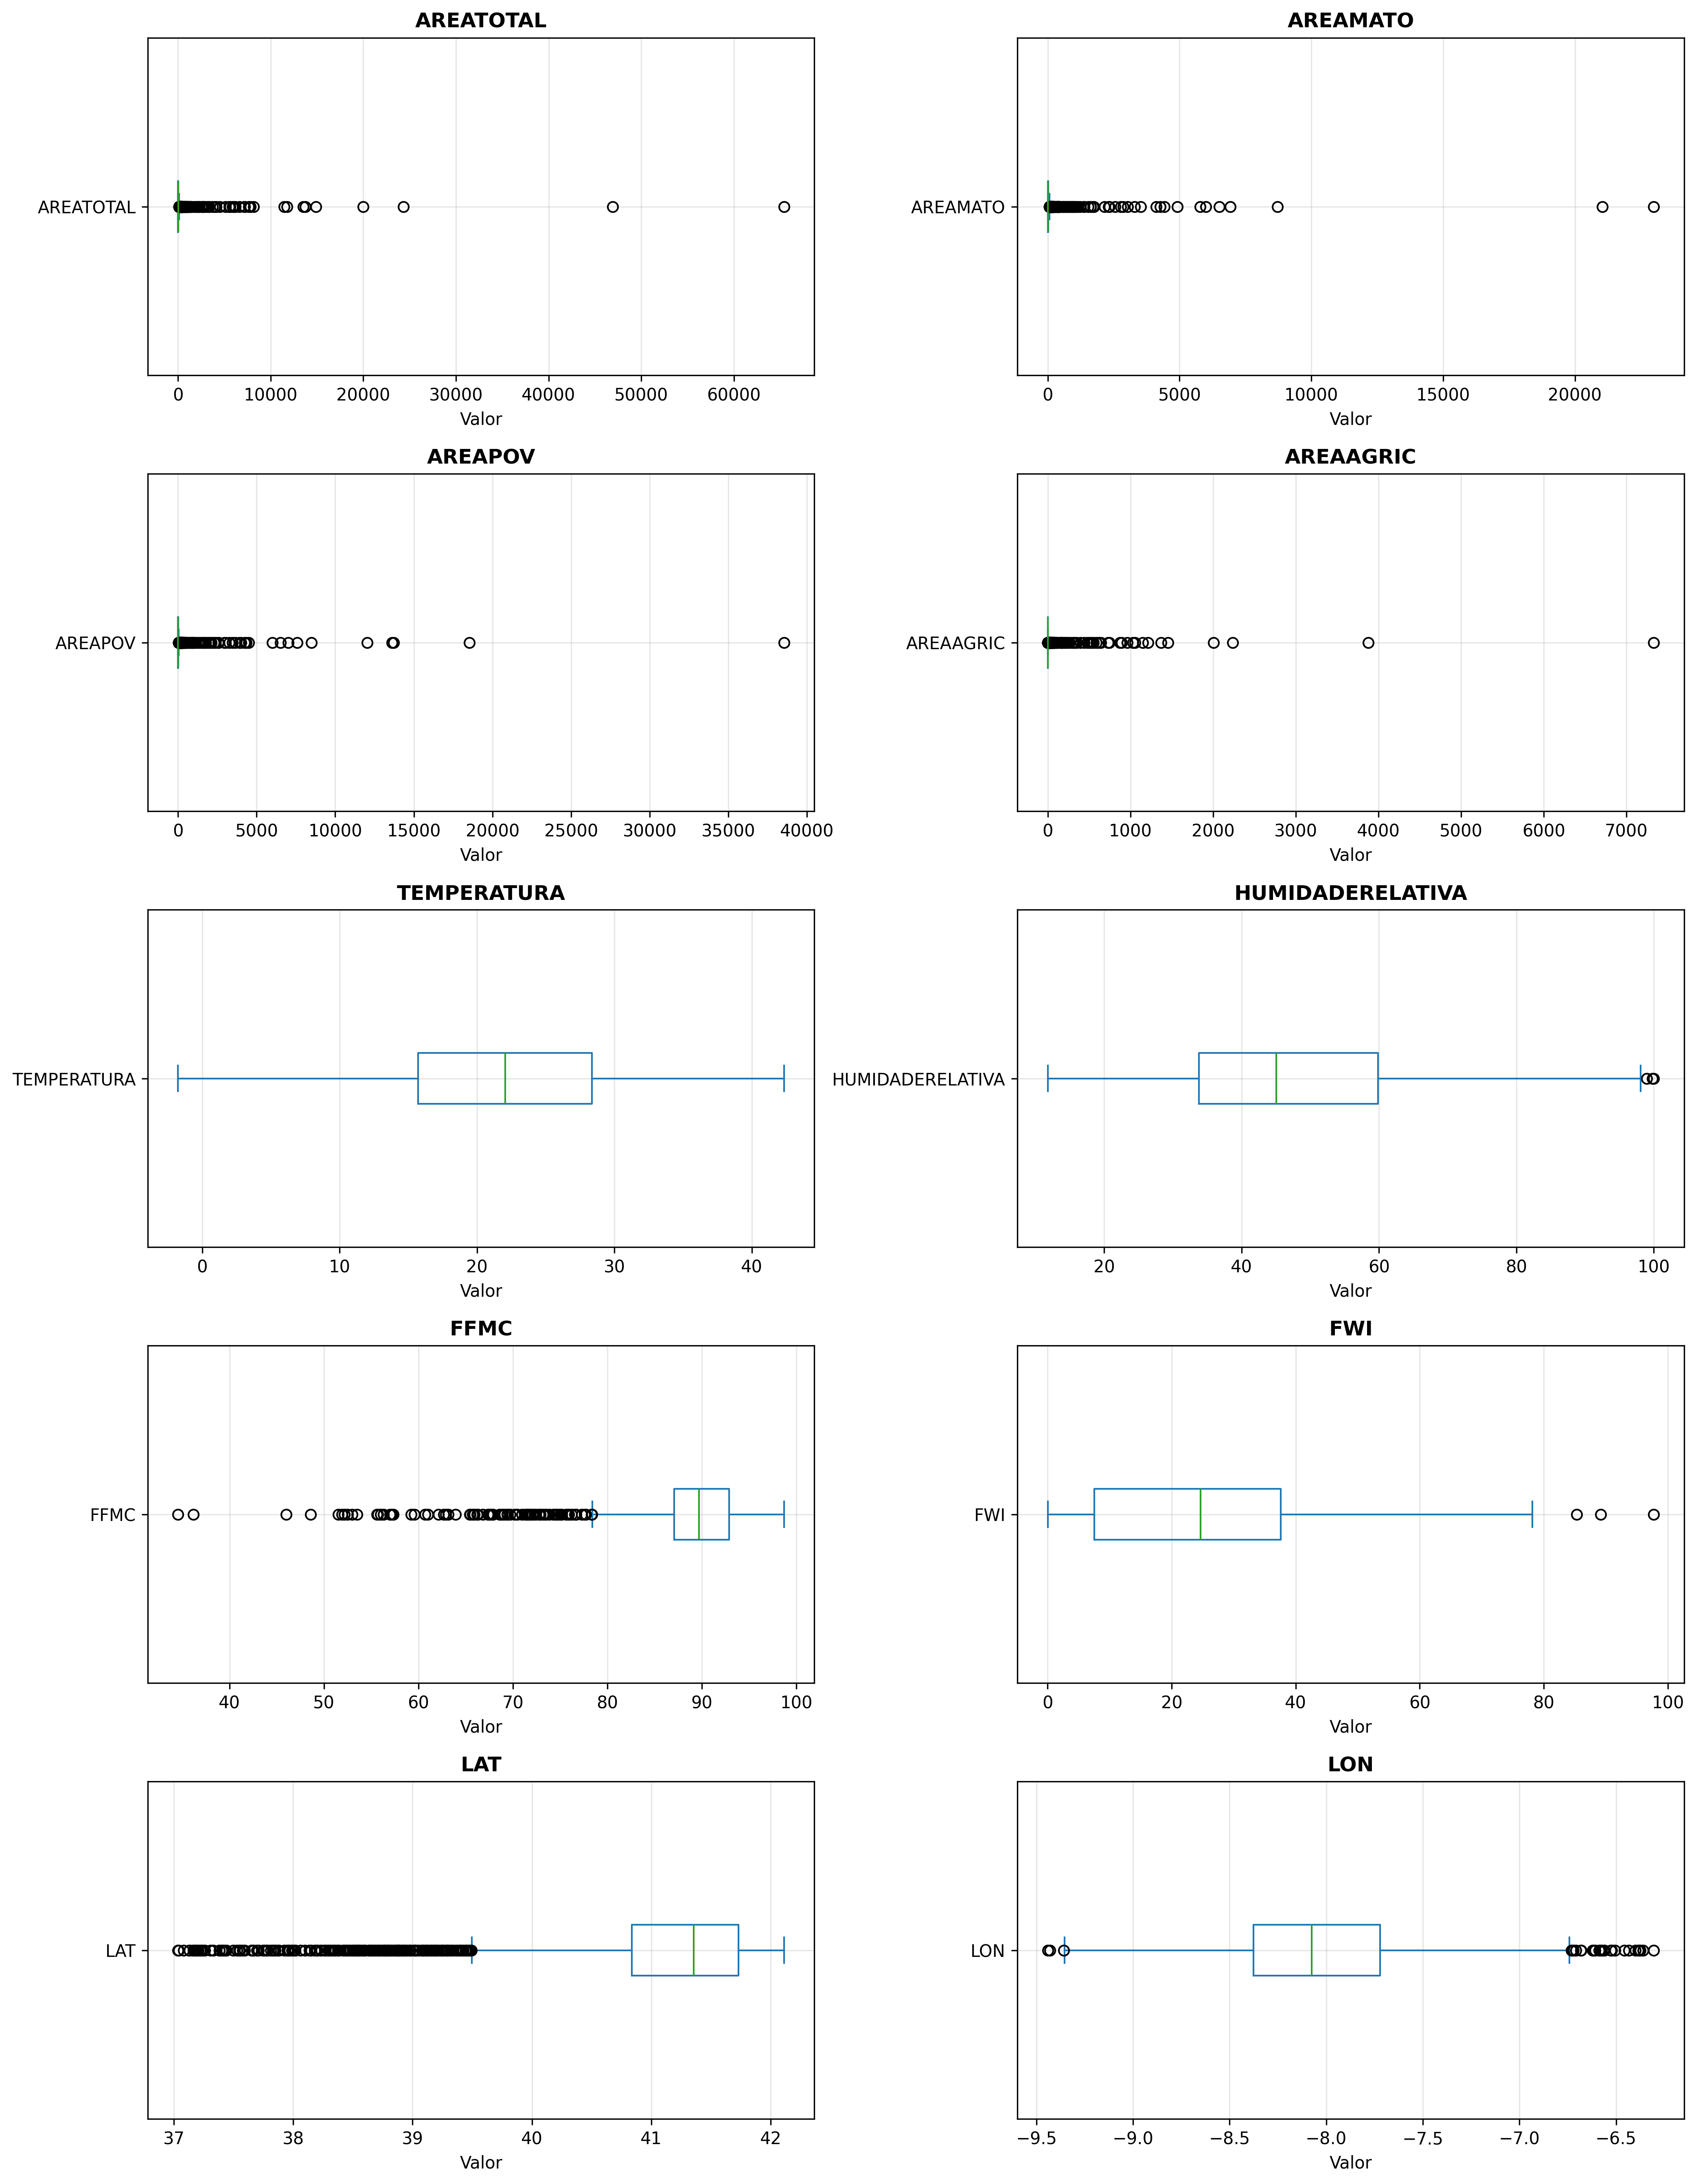
\includegraphics[width=0.8\linewidth]{imagens/07_boxplots_individuais.png}
    \caption{Bloxplpot Individuais das variáveis escolhidas do ICNF}
    \label{fig:boxplot_individuais}
\end{figure}

\textbf{Variáveis de Área Ardida (AREATOTAL, AREAMATO, AREAPOV, AREAAGRIC):} Observa-se uma forte assimetria positiva, com a maioria das ocorrências concentrada em valores baixos (pequenos incêndios) e uma cauda longa de outliers extremos correspondentes a grandes incêndios florestais. Esta distribuição reflete a natureza do fenómeno, onde eventos raros mas catastróficos têm impacto desproporcional. Os outliers superiores não são erros mas sim eventos genuínos que devem ser preservados na análise.

\textbf{Variáveis Meteorológicas:} A TEMPERATURA apresenta distribuição mais simétrica, com outliers em ambas as caudas refletindo condições meteorológicas extremas. A HUMIDADERELATIVA mostra concentração em valores médios-altos, com outliers inferiores associados a períodos de seca críticos para propagação de incêndios.

\textbf{Índices de Perigo (FFMC, FWI):} O FFMC (Fine Fuel Moisture Code) apresenta outliers superiores indicativos de condições extremas de secura de combustíveis finos. O FWI (Fire Weather Index) mostra padrão semelhante, com valores extremos sinalizando dias de perigo excecional.


\subsection{Análise da Distribuição Espacial das Ocorrências}
\label{Analise_da_distribuicao_espacial_das_ocorrencias}
A análise da distribuição geográfica por distrito (Figura \ref{fig:20Distritos}) revela um grande padrão de concentração espacial. Os distritos do interior Norte e Centro do país dominam claramente as estatísticas, refletindo a conjugação de fatores como maior cobertura florestal, condições climáticas mais propícias, e características sócio-económicas das populações rurais.

Os três distritos com maior incidência acumulam uma proporção significativa do total de ocorrências, evidenciando a necessidade de políticas de prevenção geograficamente diferenciadas. Esta concentração justifica também a inclusão da dimensão geográfica como eixo central de análise no Data Warehouse.

\begin{figure}
    \centering
    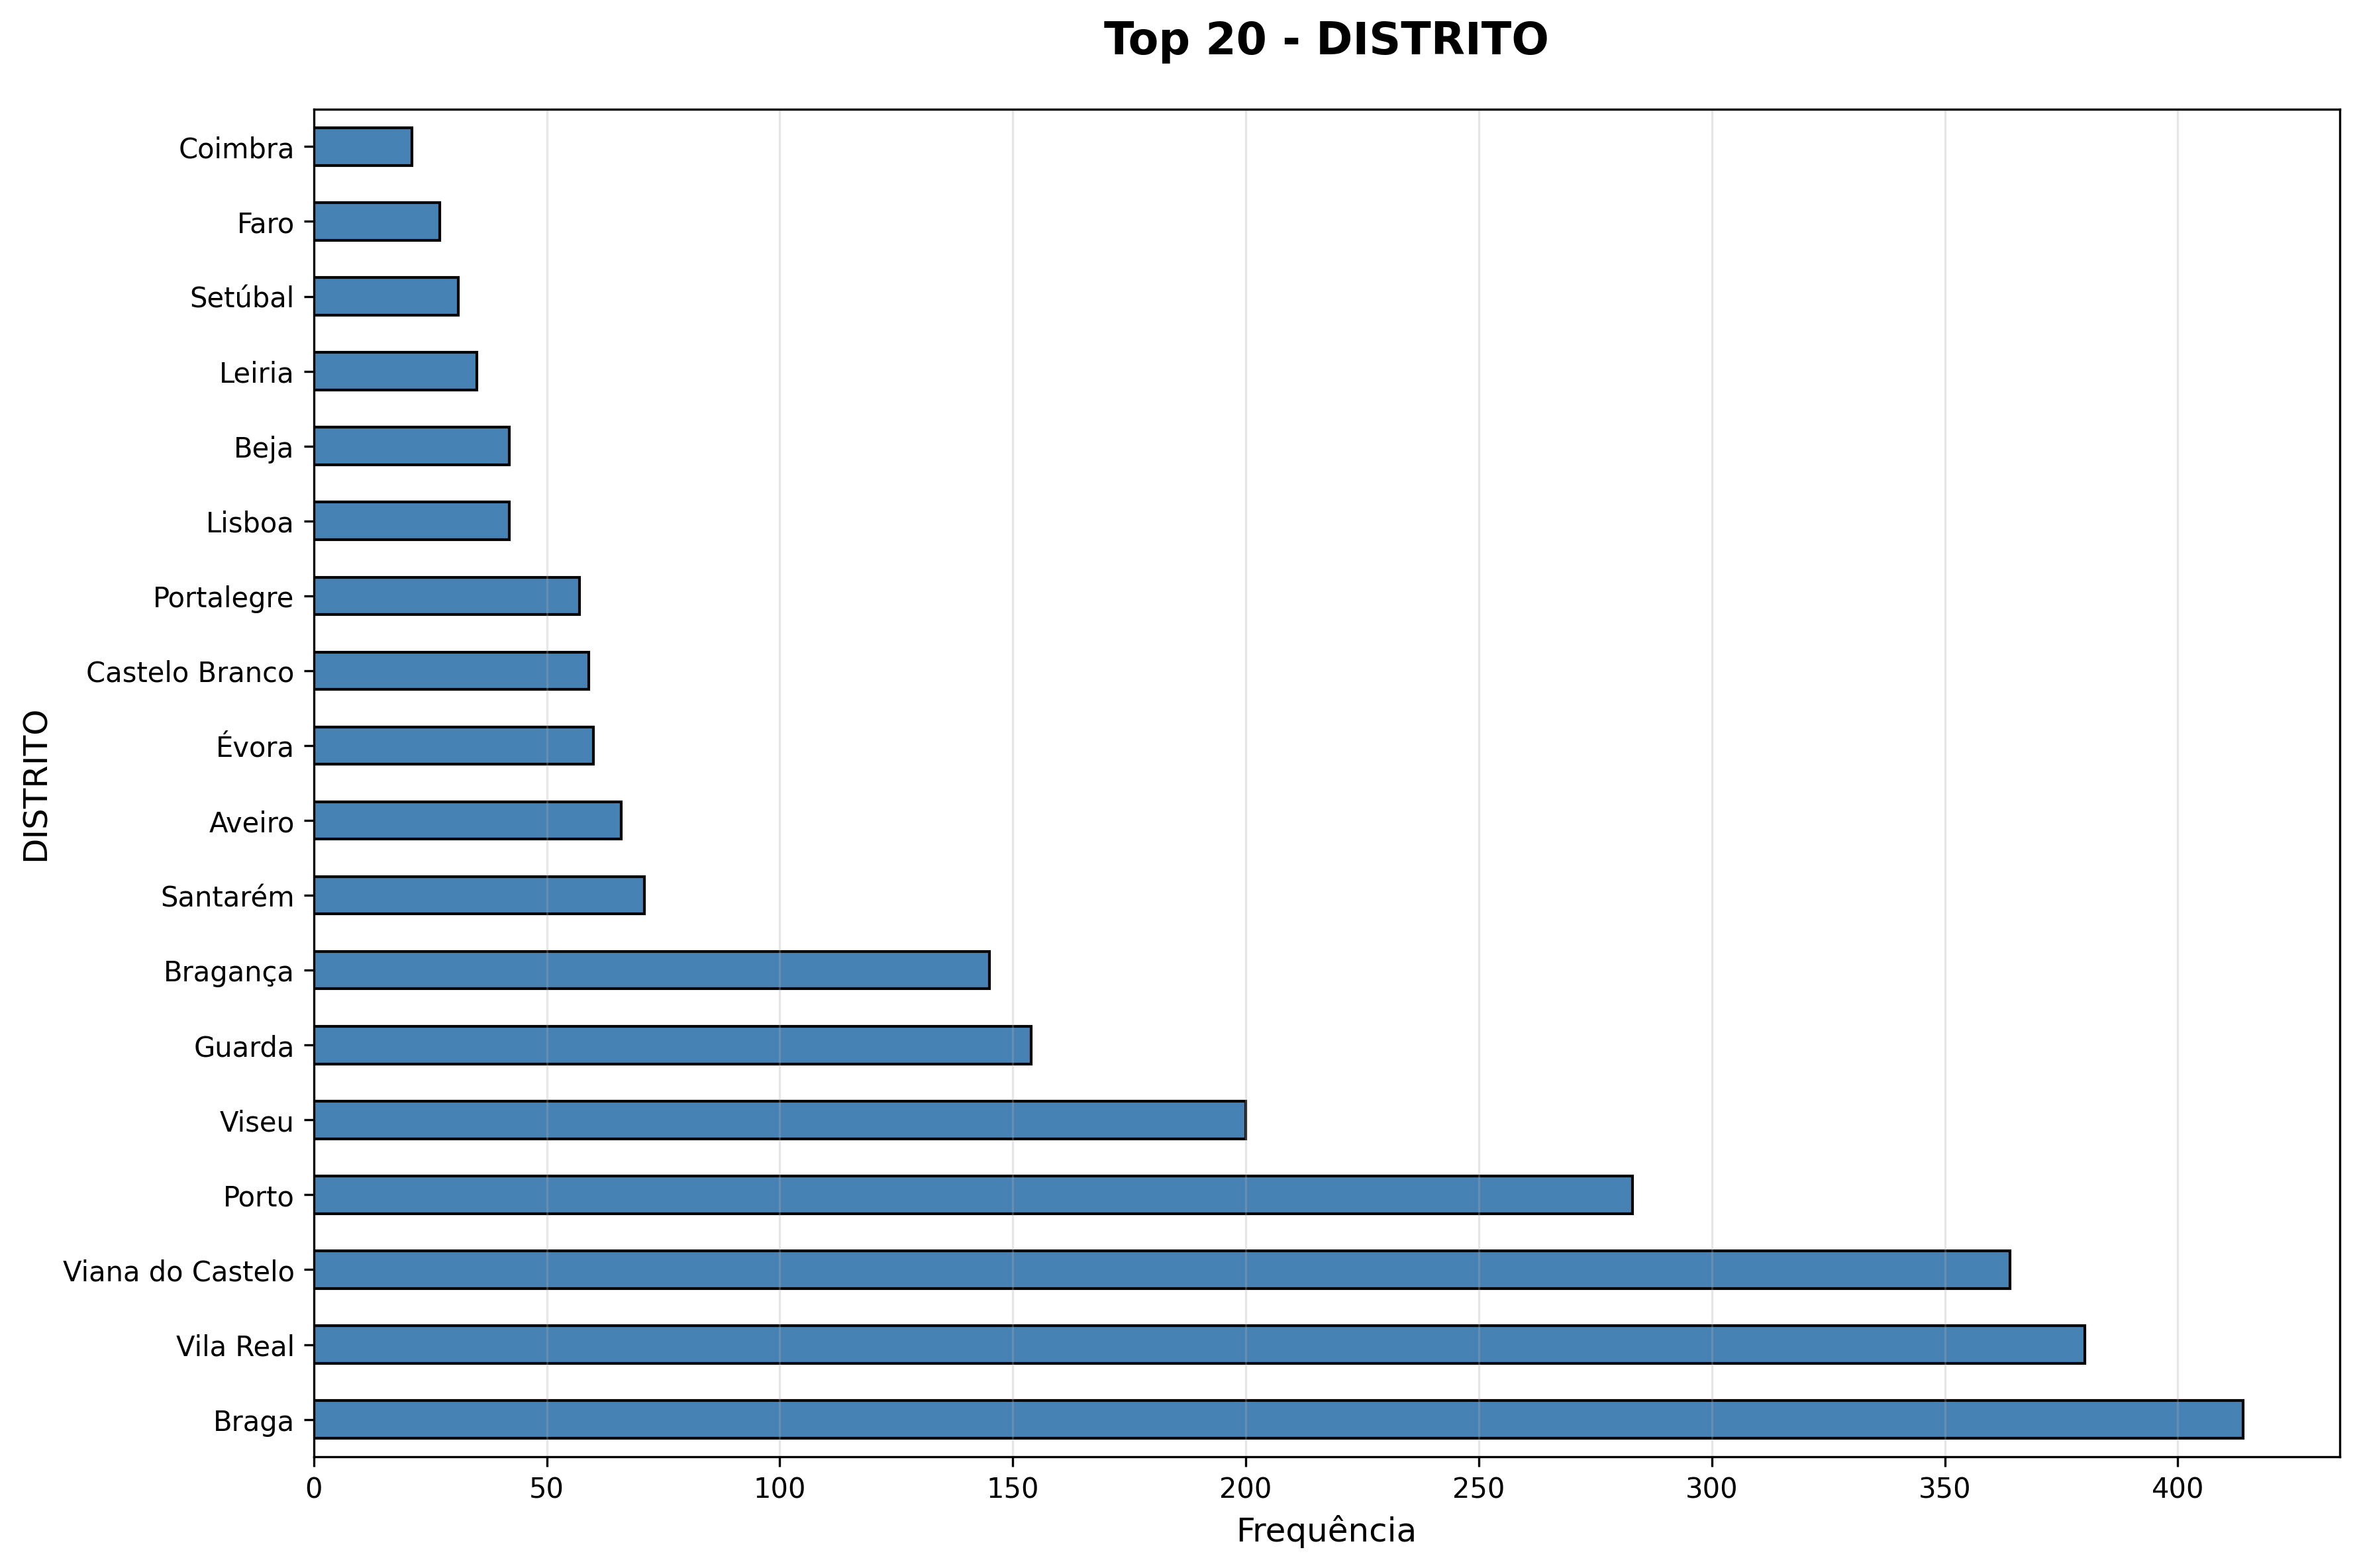
\includegraphics[width=0.7\linewidth]{imagens/03_grafico_DISTRITO.png}
    \caption{Top 20 distritos com maior frequência de ocorrências de incêndio}
    \label{fig:20Distritos}
\end{figure}

A desagregação ao nível da freguesia (Figura \ref{fig:20Freguesias}) revela hotspots localizados onde a recorrência é particularmente elevada. Esta granularidade é essencial para:

\begin{itemize}
    \item Identificação de áreas prioritárias para investimento em prevenção
    \item Análise de padrões de reincidência espacial
    \item Correlação com características locais (tipo de vegetação, densidade populacional, acessibilidades)
\end{itemize}

Observa-se que as freguesias com maior número de ocorrências não coincidem necessariamente com as de maior área ardida, sugerindo diferenças na efeciência de combate ou em características de propagação.

\begin{figure}
    \centering
    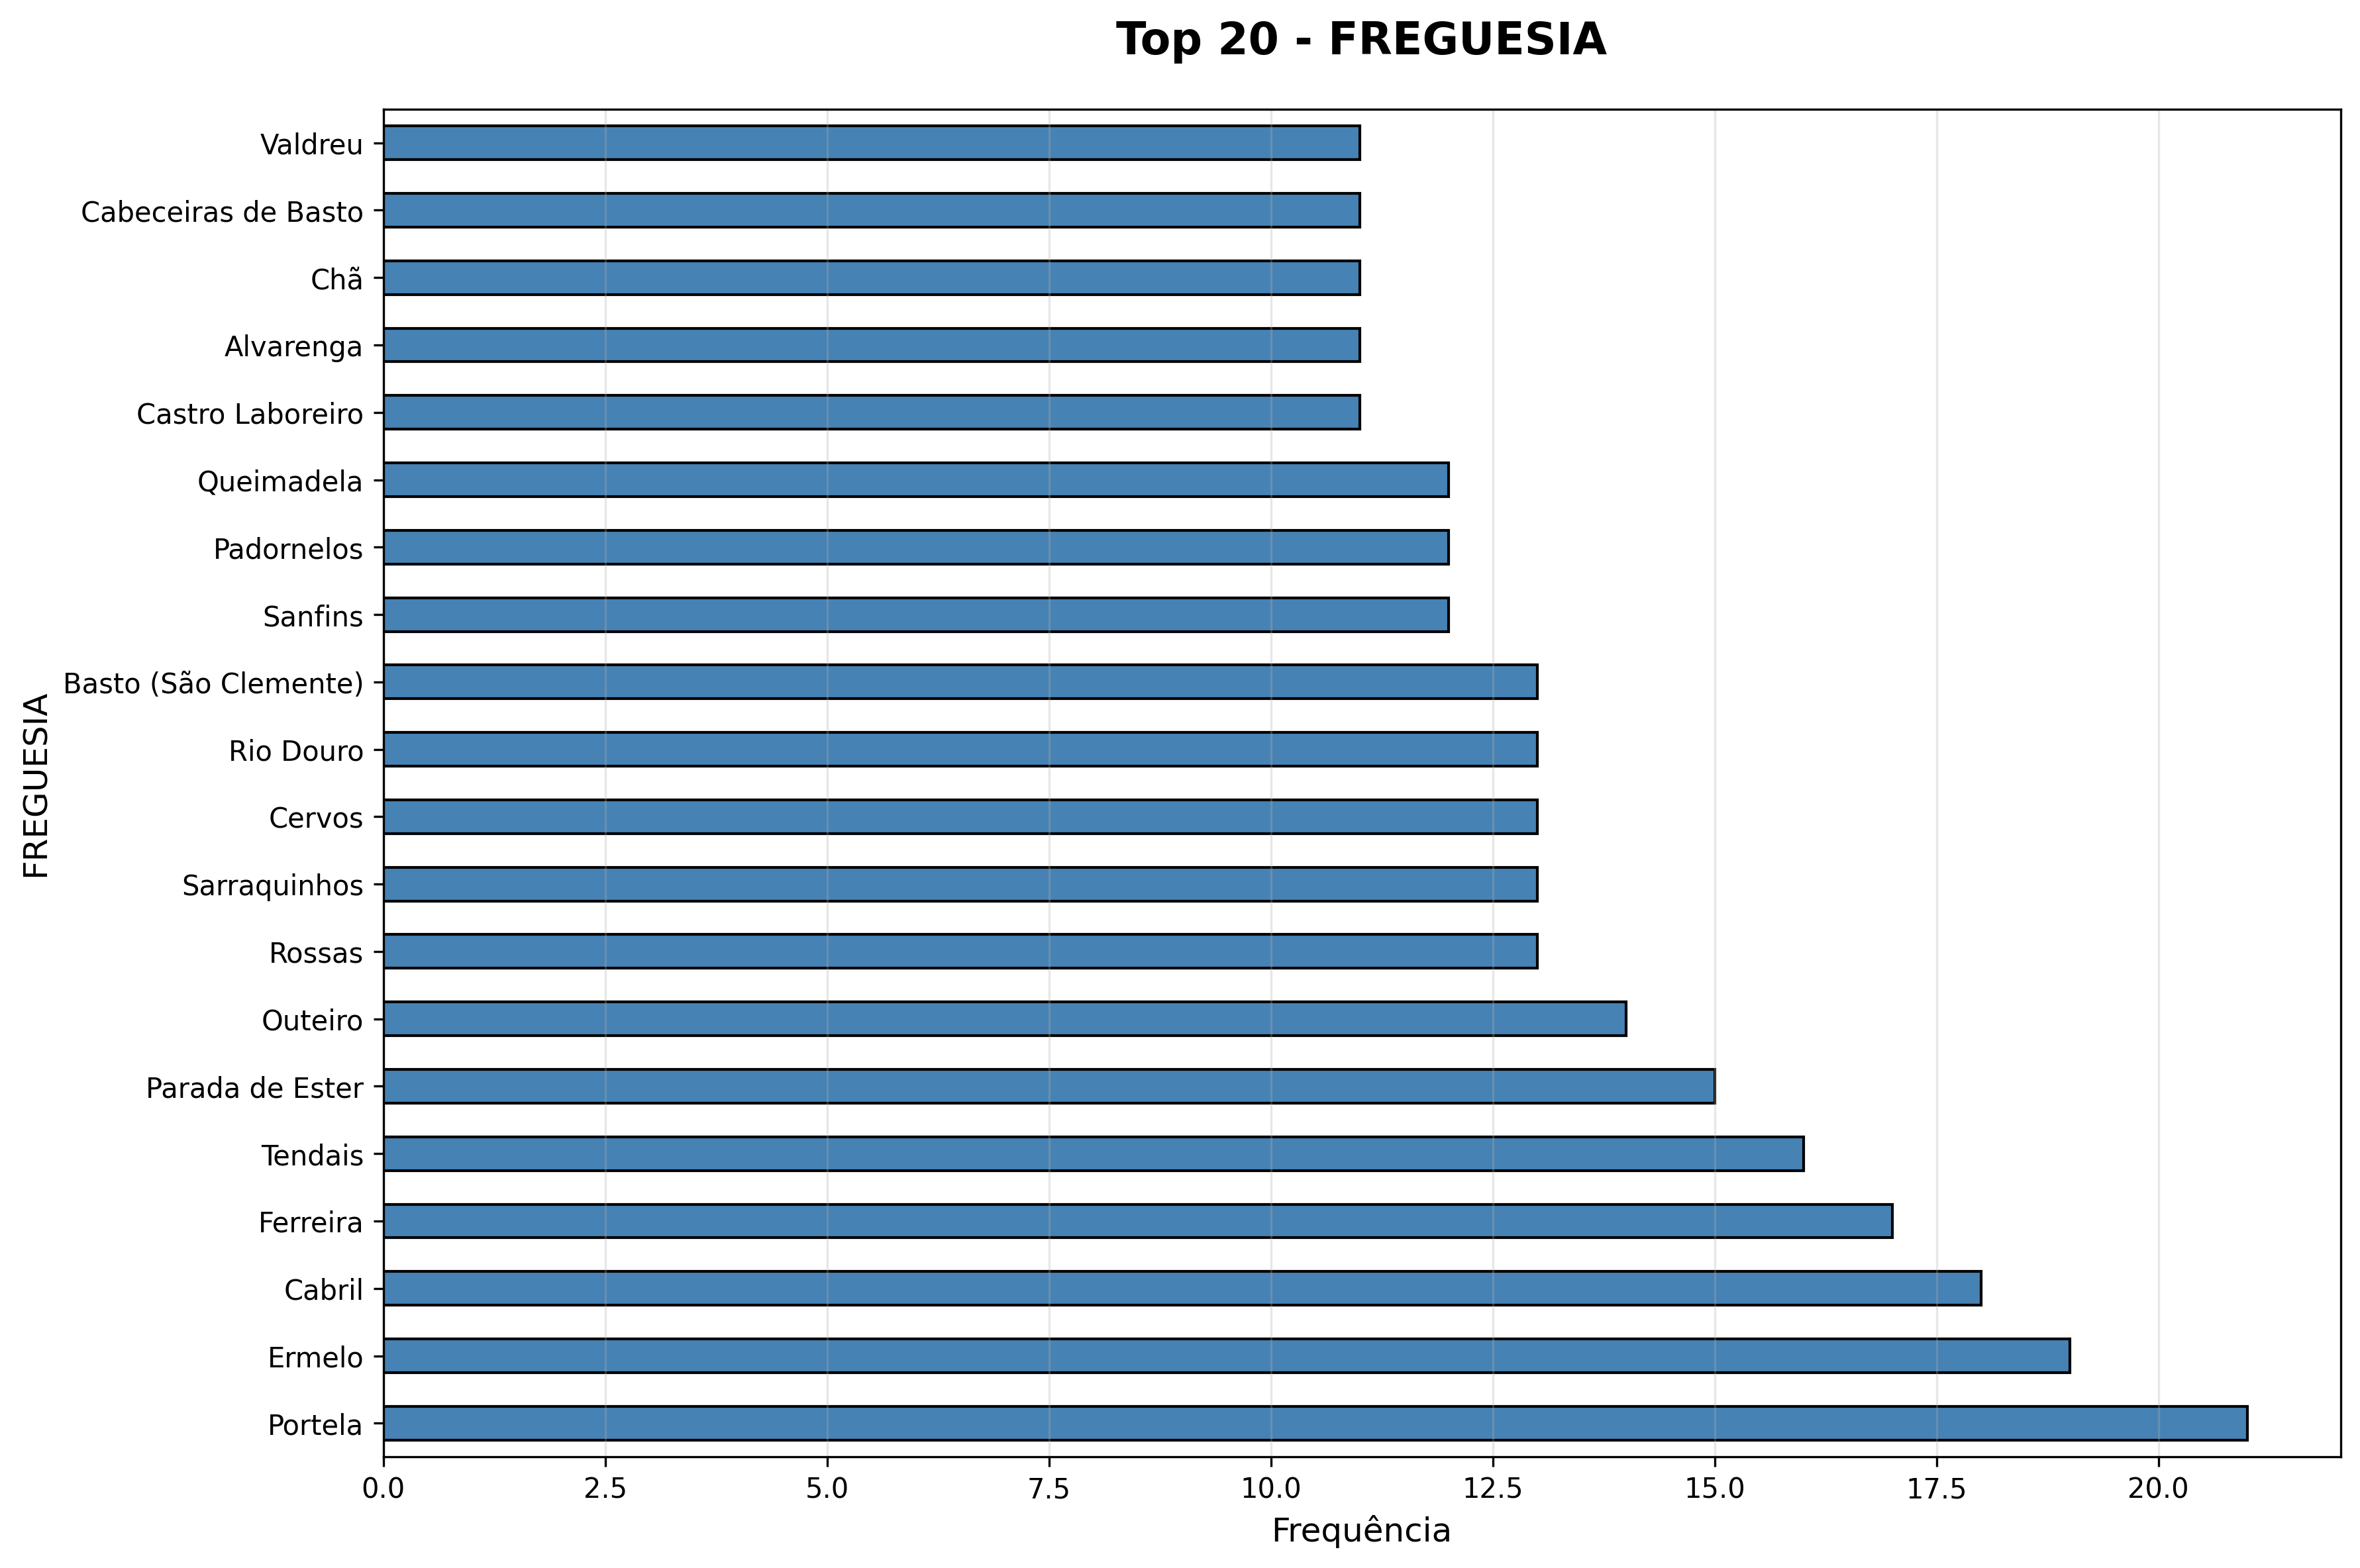
\includegraphics[width=0.7\linewidth]{imagens/03_grafico_FREGUESIA.png}
    \caption{Top 20 freguesias com maior frequência de ocorrências de incêndio} 
    \label{fig:20Freguesias}
\end{figure}

\subsection{Análise Causal} \label{Analise_Causal}
A análise de causas (Figura \ref{fig:20tipoCausa}) constitui uma das dimensões mais relevantes para políticas públicas. O gráfico evidencia a distribuição entre causas humanas (intencionais, negligentes, acidentais) e causas naturais (principalmente raios).

A predominância de causas humanas sobre naturais, caso verificada, sublinha a importância de campanhas de sensibilização e fiscalização. A categoria "Desconhecida" ou "Em investigação" pode representar uma limitação dos dados que deve ser considerada na interpretação dos resultados analíticos.

\begin{figure}
    \centering
    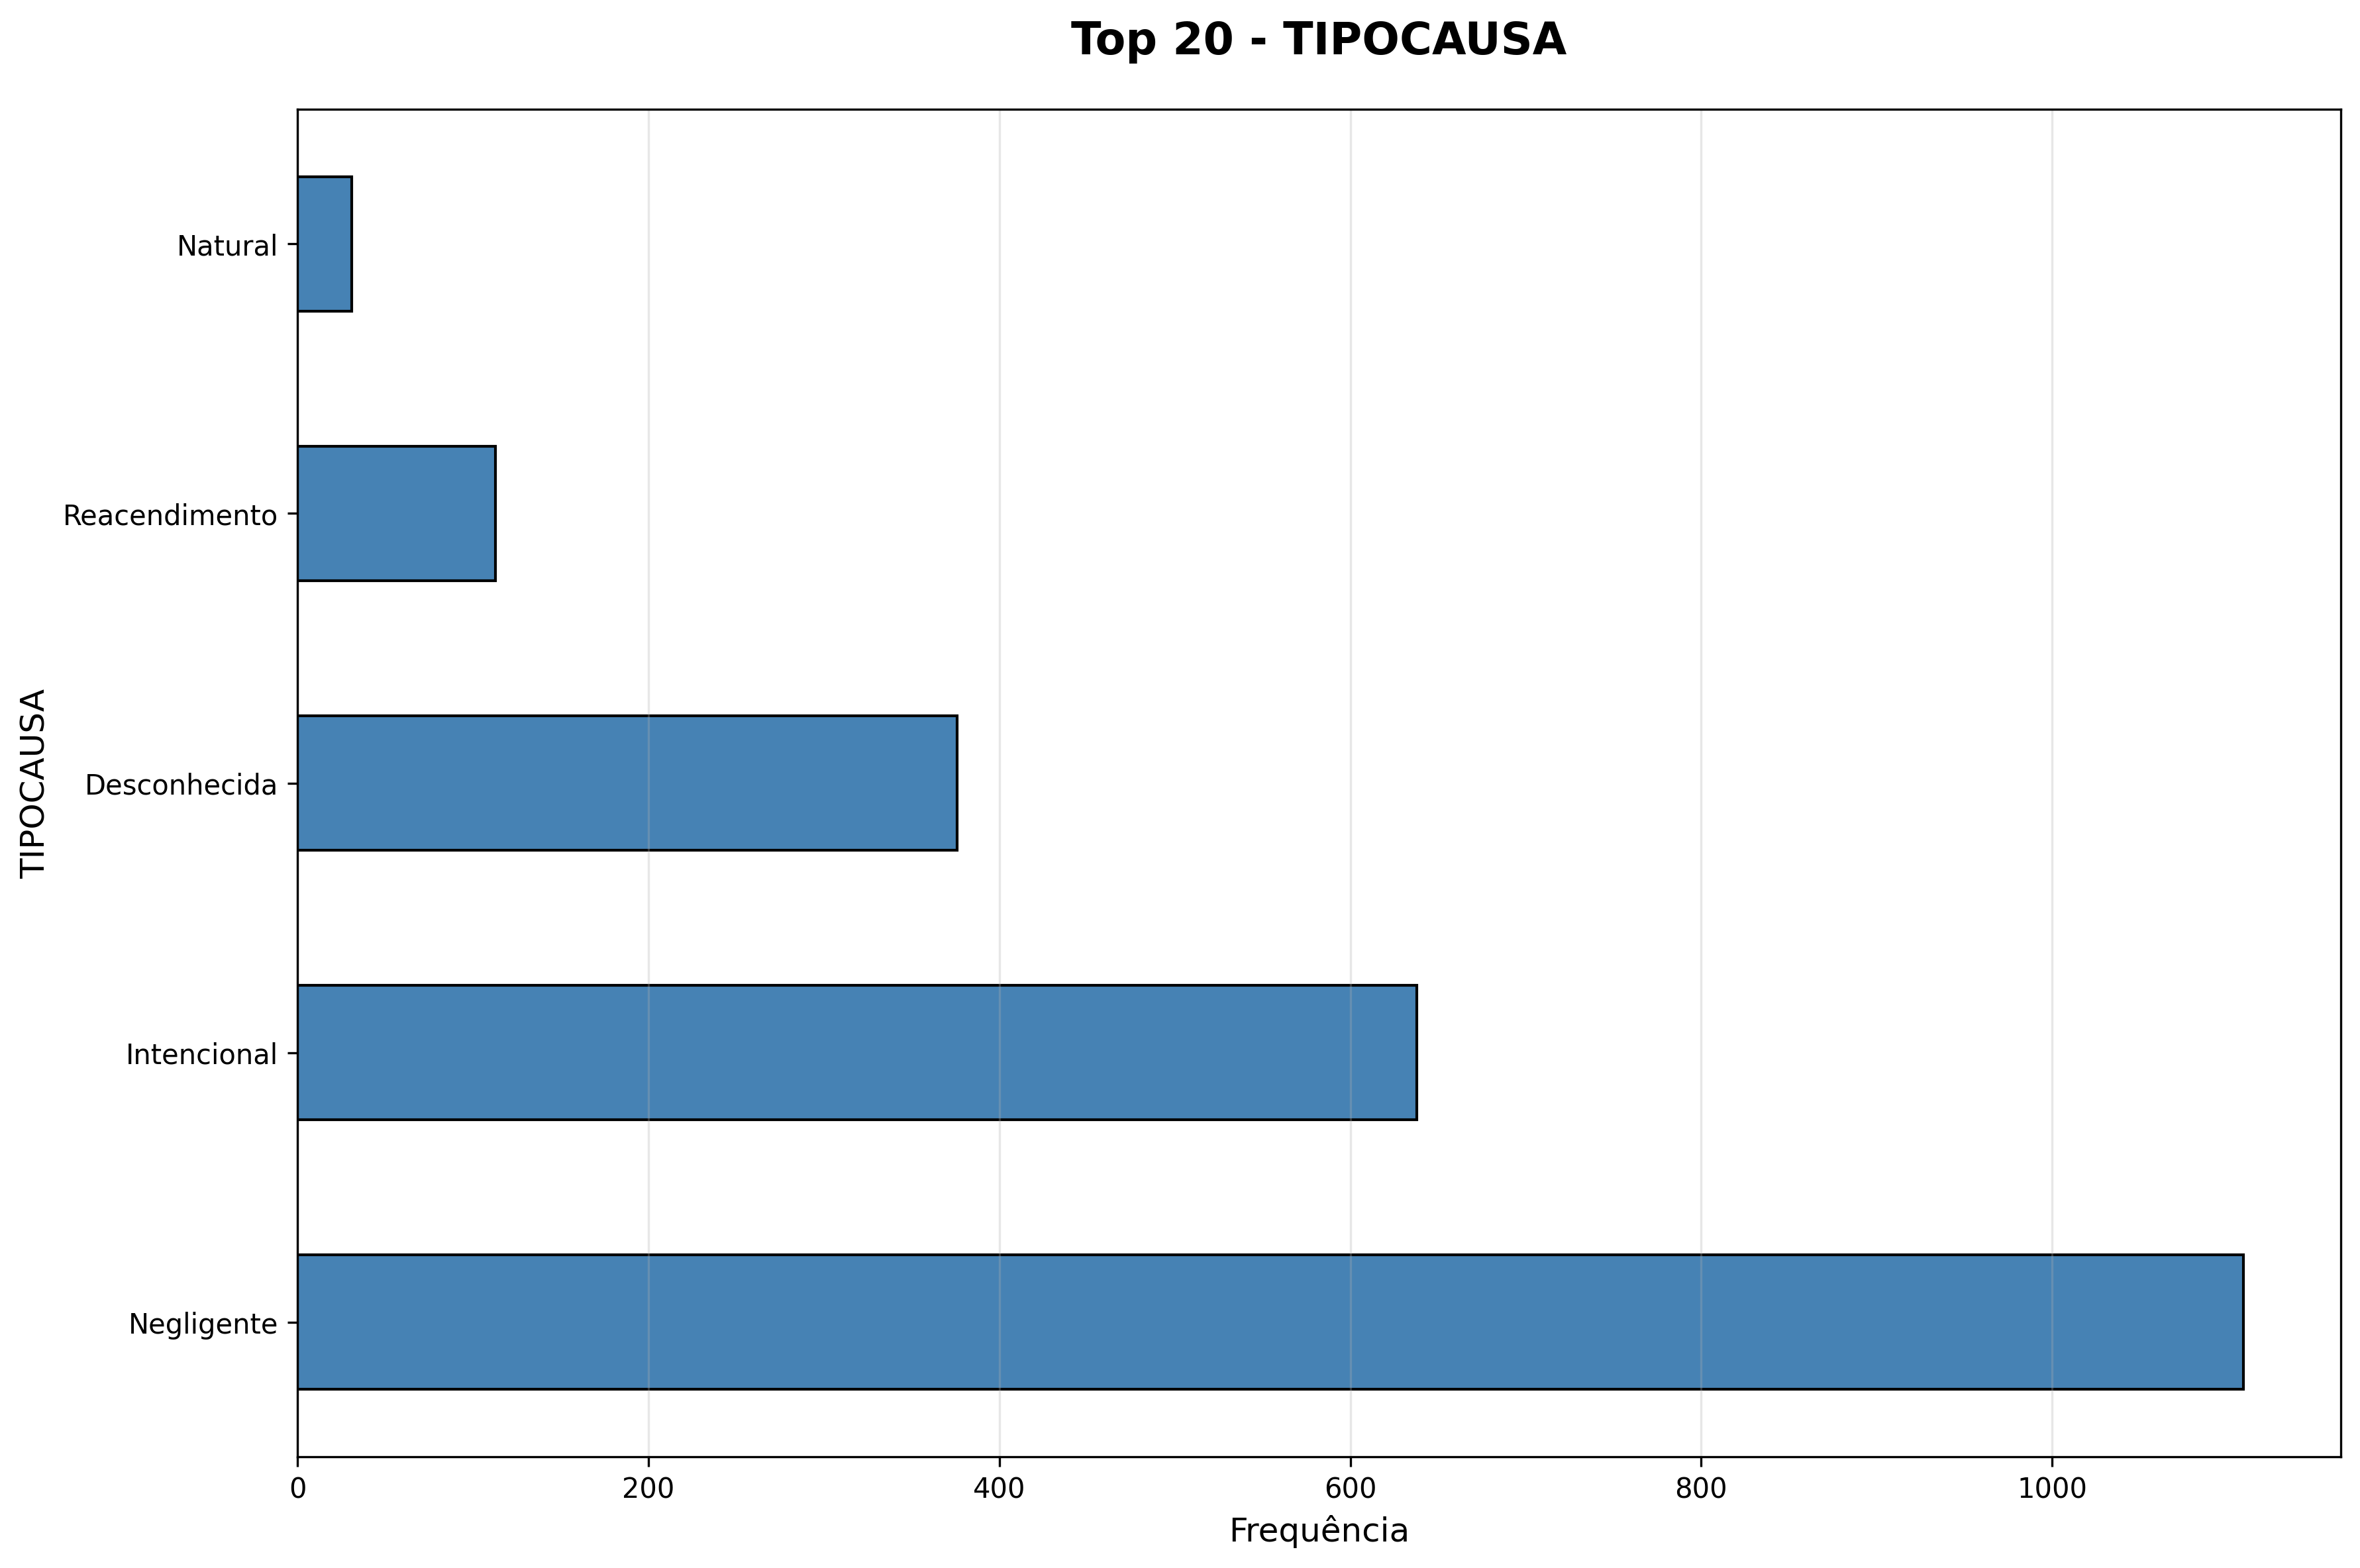
\includegraphics[width=0.7\linewidth]{imagens/03_grafico_TIPOCAUSA.png}
    \caption{Distribuição das Ocorrências por Tipo de Causa} \label{fig:20tipoCausa}
\end{figure}

Algo a realçar, é que tanto nesta secção como na secção \ref{Analise_da_distribuicao_espacial_das_ocorrencias} não foi realizado nenhum tipo de tratamento categórico nas variáveis antes de formular os gráficos de barras. E mesmo sem esse tratamento, não apareceram variáveis repetidas com nomes ligeiramente diferentes, isso significa que não existe nenhum tipo de incoerência nos valores das variáveis que iram obrigar a futura utilização das tabelas de dicionário.


\subsection{Relações entre as variáveis}
A matriz de correlações (Figura \ref{fig:correlacoes}) revela as interdependências entre variáveis numéricas, essenciais para:

\begin{figure}
    \centering
    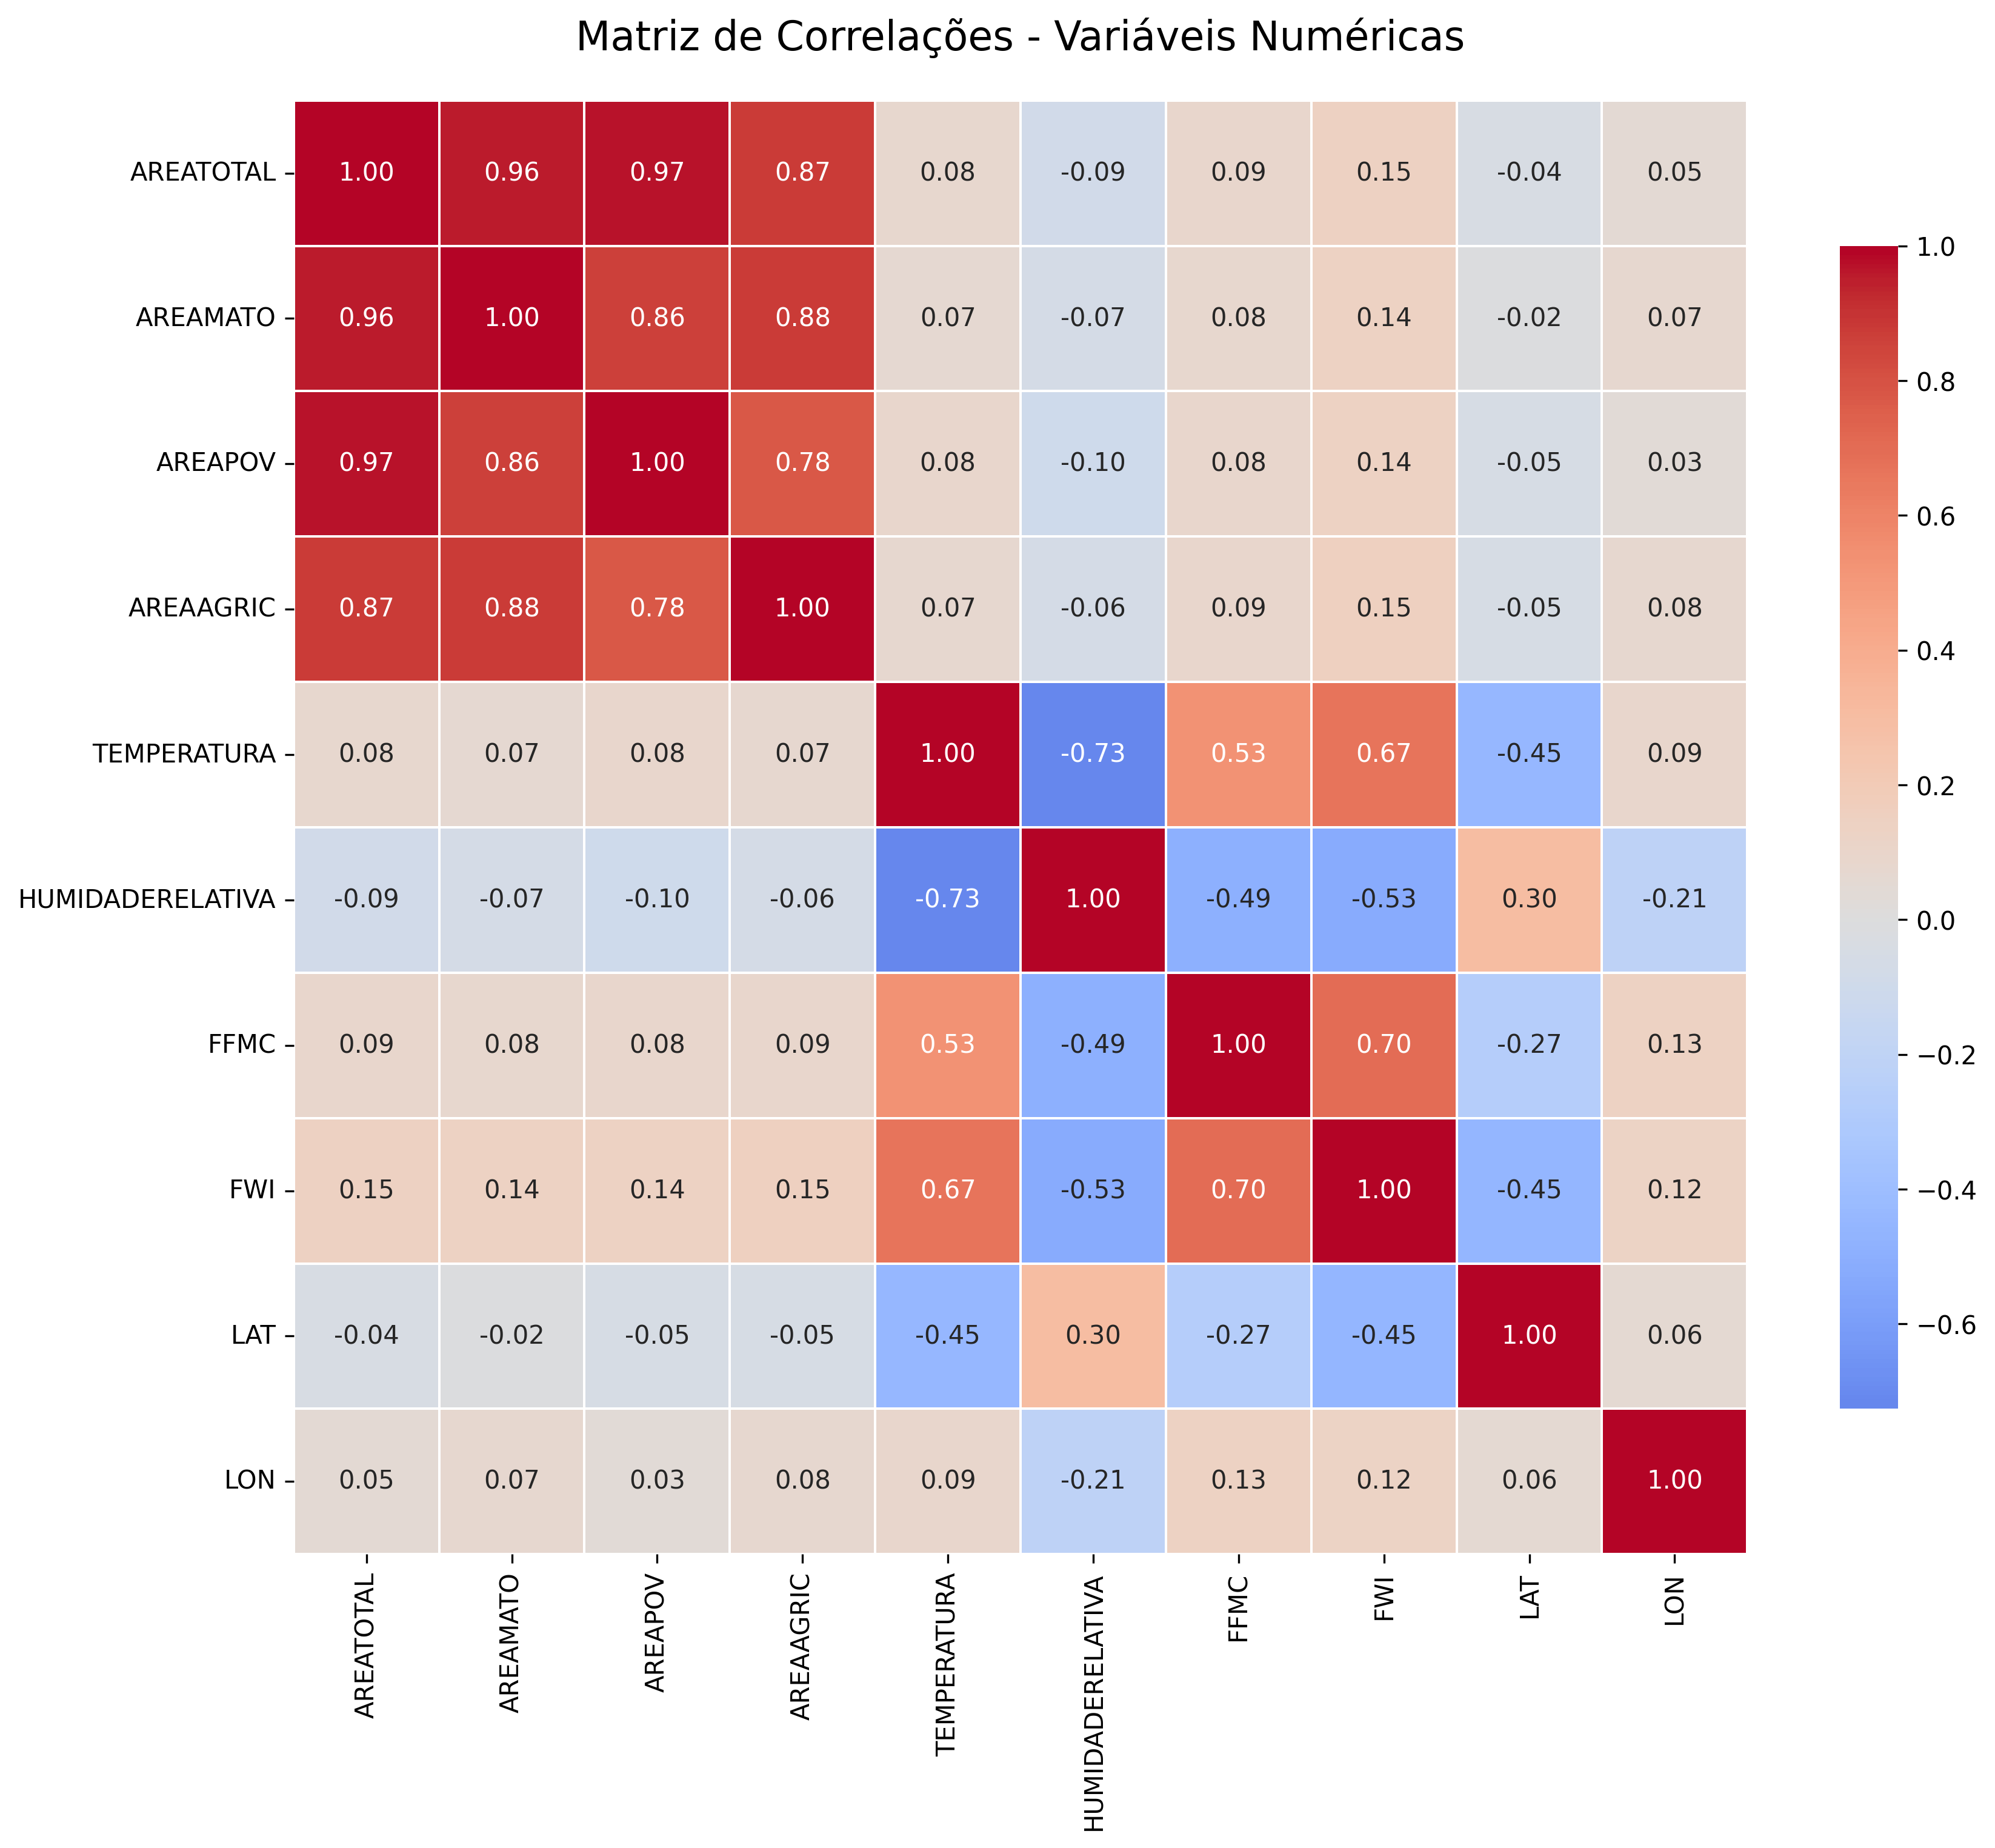
\includegraphics[width=0.8\linewidth]{imagens/06_correlacoes.png}
    \caption{Matriz de correlações entre variáveis numéricas}
    \label{fig:correlacoes}
\end{figure}

\subsubsection{Correlações Fortes Esperadas:}

\begin{itemize}
    \item \textbf{AREATOTAL vs. AREAMATO/AREAPOV:} Correlações positivas fortes (r > 0.7), indicando que estes são os principais componentes contribuidores para a área total. A magnitude relativa das correlações indica qual tipo de vegetação domina.
    \item \textbf{TEMPERATURA vs. HUMIDADERELATIVA:} Correlação negativa esperada (r < -0.5), refletindo a relação física inversa entre estas variáveis.
    \item \textbf{FFMC vs. FWI:} Correlação positiva forte, dado que o FFMC é um dos componentes do índice compósito FWI.
\end{itemize}


\subsubsection{Correlações Moderadas de Interesse:}
\begin{itemize}
    \item \textbf{Índices meteorológicos vs. Área ardida:} Correlações positivas moderadas sugerem que condições meteorológicas adversas contribuem para incêndios maiores, mas não determinam completamente a severidade (outros fatores como tempo de resposta e meios disponíveis são relevantes).
    \item \textbf{TEMPERATURA vs. Área ardida: }Correlação positiva esperada, validando o papel das ondas de calor na severidade dos incêndios.
\end{itemize}

